\clearpage
\subsection{Подготовка клиентов}

Для того, чтобы подготовить к работе терминал, нужно установить ОС, RDP-клиент, и 
настроить автоматическое подключение к серверу.

С официального сайта \cite{ref:raspbian} необходимо скачать iso-образ Raspbian, версии
Lite без рабочего стола. Для установки ОС на microSD карту используется Etcher
\cite{ref:etcher}. Выбирается загруженный образ, нужный носитель и производится запись
(см. рисунок~\ref{pic:rpi-etcher}).

\begin{figure}[h]
    \center
    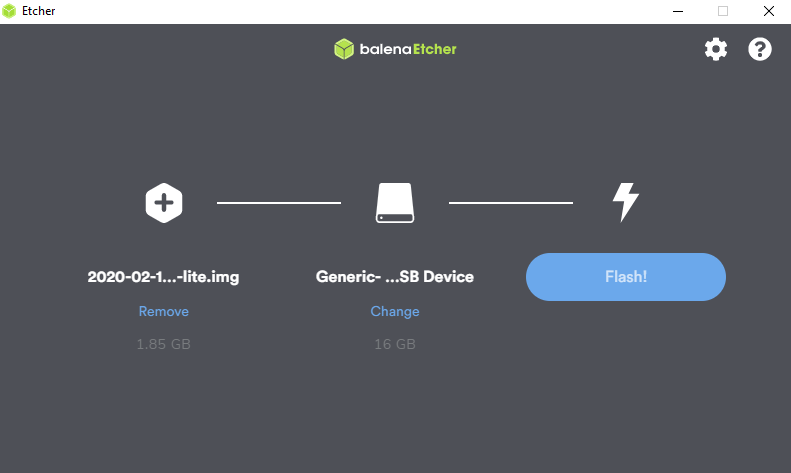
\includegraphics[width=\linewidth]{rpi-etcher}
    \caption{Запись iso на SD-карту с помощью Etcher}
    \label{pic:rpi-etcher}
\end{figure}

\begin{figure}[h]
    \center
    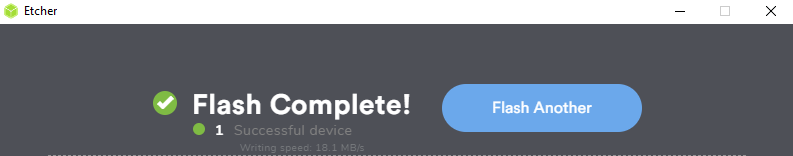
\includegraphics[width=\linewidth]{rpi-etcher-complete}
    \caption{Подтверждение успешной записи}
    \label{pic:rpi-etcher-complete}
\end{figure}

\begin{figure}[h]
    \center
    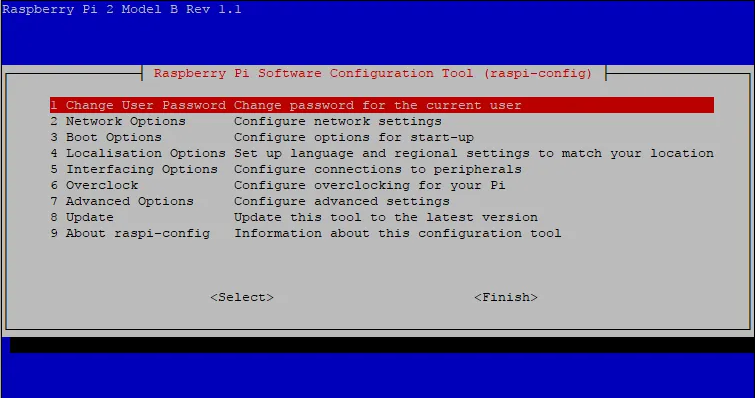
\includegraphics[width=\linewidth]{raspi-config}
    \caption{Окно утилиты \texttt{raspi-config}}
    \label{pic:raspi-config}
\end{figure}

После подтверждения успешной записи (см. рисунок~\ref{pic:rpi-etcher-complete}) можно
выходить из программы. Далее microSD–карта устанавливается в Raspberry Pi, подключаются
источник питания, сетевой кабель (на данном этапе нужен доступ в Интернет), клавиатура 
и монитор. После загрузки необходимо авторизоваться (по умолчанию логин — 
\texttt{pi}, пароль — \texttt{raspberry}). Теперь доступен режим работы с командной
строкой.

Нужно установить раскладку клавиатуры \texttt{en\_US.UTF-8} и выбрать часовой пояс. Это
можно сделать с помощью программы \texttt{raspi-config} (см.
рисунок~\ref{pic:raspi-config}) в пункте Localisation Options.  Также необходимо сменить
пароль для пользователя \texttt{pi} (Change User Password), а также выбрать режим
автоматического входа в систему (Boot Options — Desktop/CLI — Console autologin).

Обновление каталога ПО и установка нужных пакетов выполняется следующими командами:
\begin{verbatim}
sudo apt update && sudo apt upgrade
sudo apt install --no-install-recommends xserver-xorg \
    x11-xserver-utils xinit openbox
sudo apt install freerdp2-x11 pulseaudio
\end{verbatim}

Теперь нужно настроить действия при загрузке сеанса. Редактируется файл
\texttt{/etc/xdg/openbox/autostart}, в котором будет вызываться RDP-клиент:
\begin{verbatim}
# Отключить все функции энергосбережения
xset s off
xset s noblank
xset -dpms

# Завершение сеанса по Ctrl-Alt-Backspace
setxkbmap -option terminate:ctrl_alt_bksp

# Запуск RDP с нужными параметрами
while true; do
  xfreerdp /fonts /bpp:15 /f /audio-mode:0 /u:[user] /p:[password] \
    /v:[ip] /gdi:hw /sound:sys:pulse /gfx:rfx /rfx-mode:video \
    +bitmap-cache +offscreen-cache -clipboard
done
\end{verbatim}

Нужно заменить поля в квадратных скобках на пользователя, пароль и IP-адрес сервера.
Теперь можно проверить работоспособность системы, загрузившись в графический режим:
\begin{verbatim}
startx --
\end{verbatim}

\begin{figure}[p]
    \center
    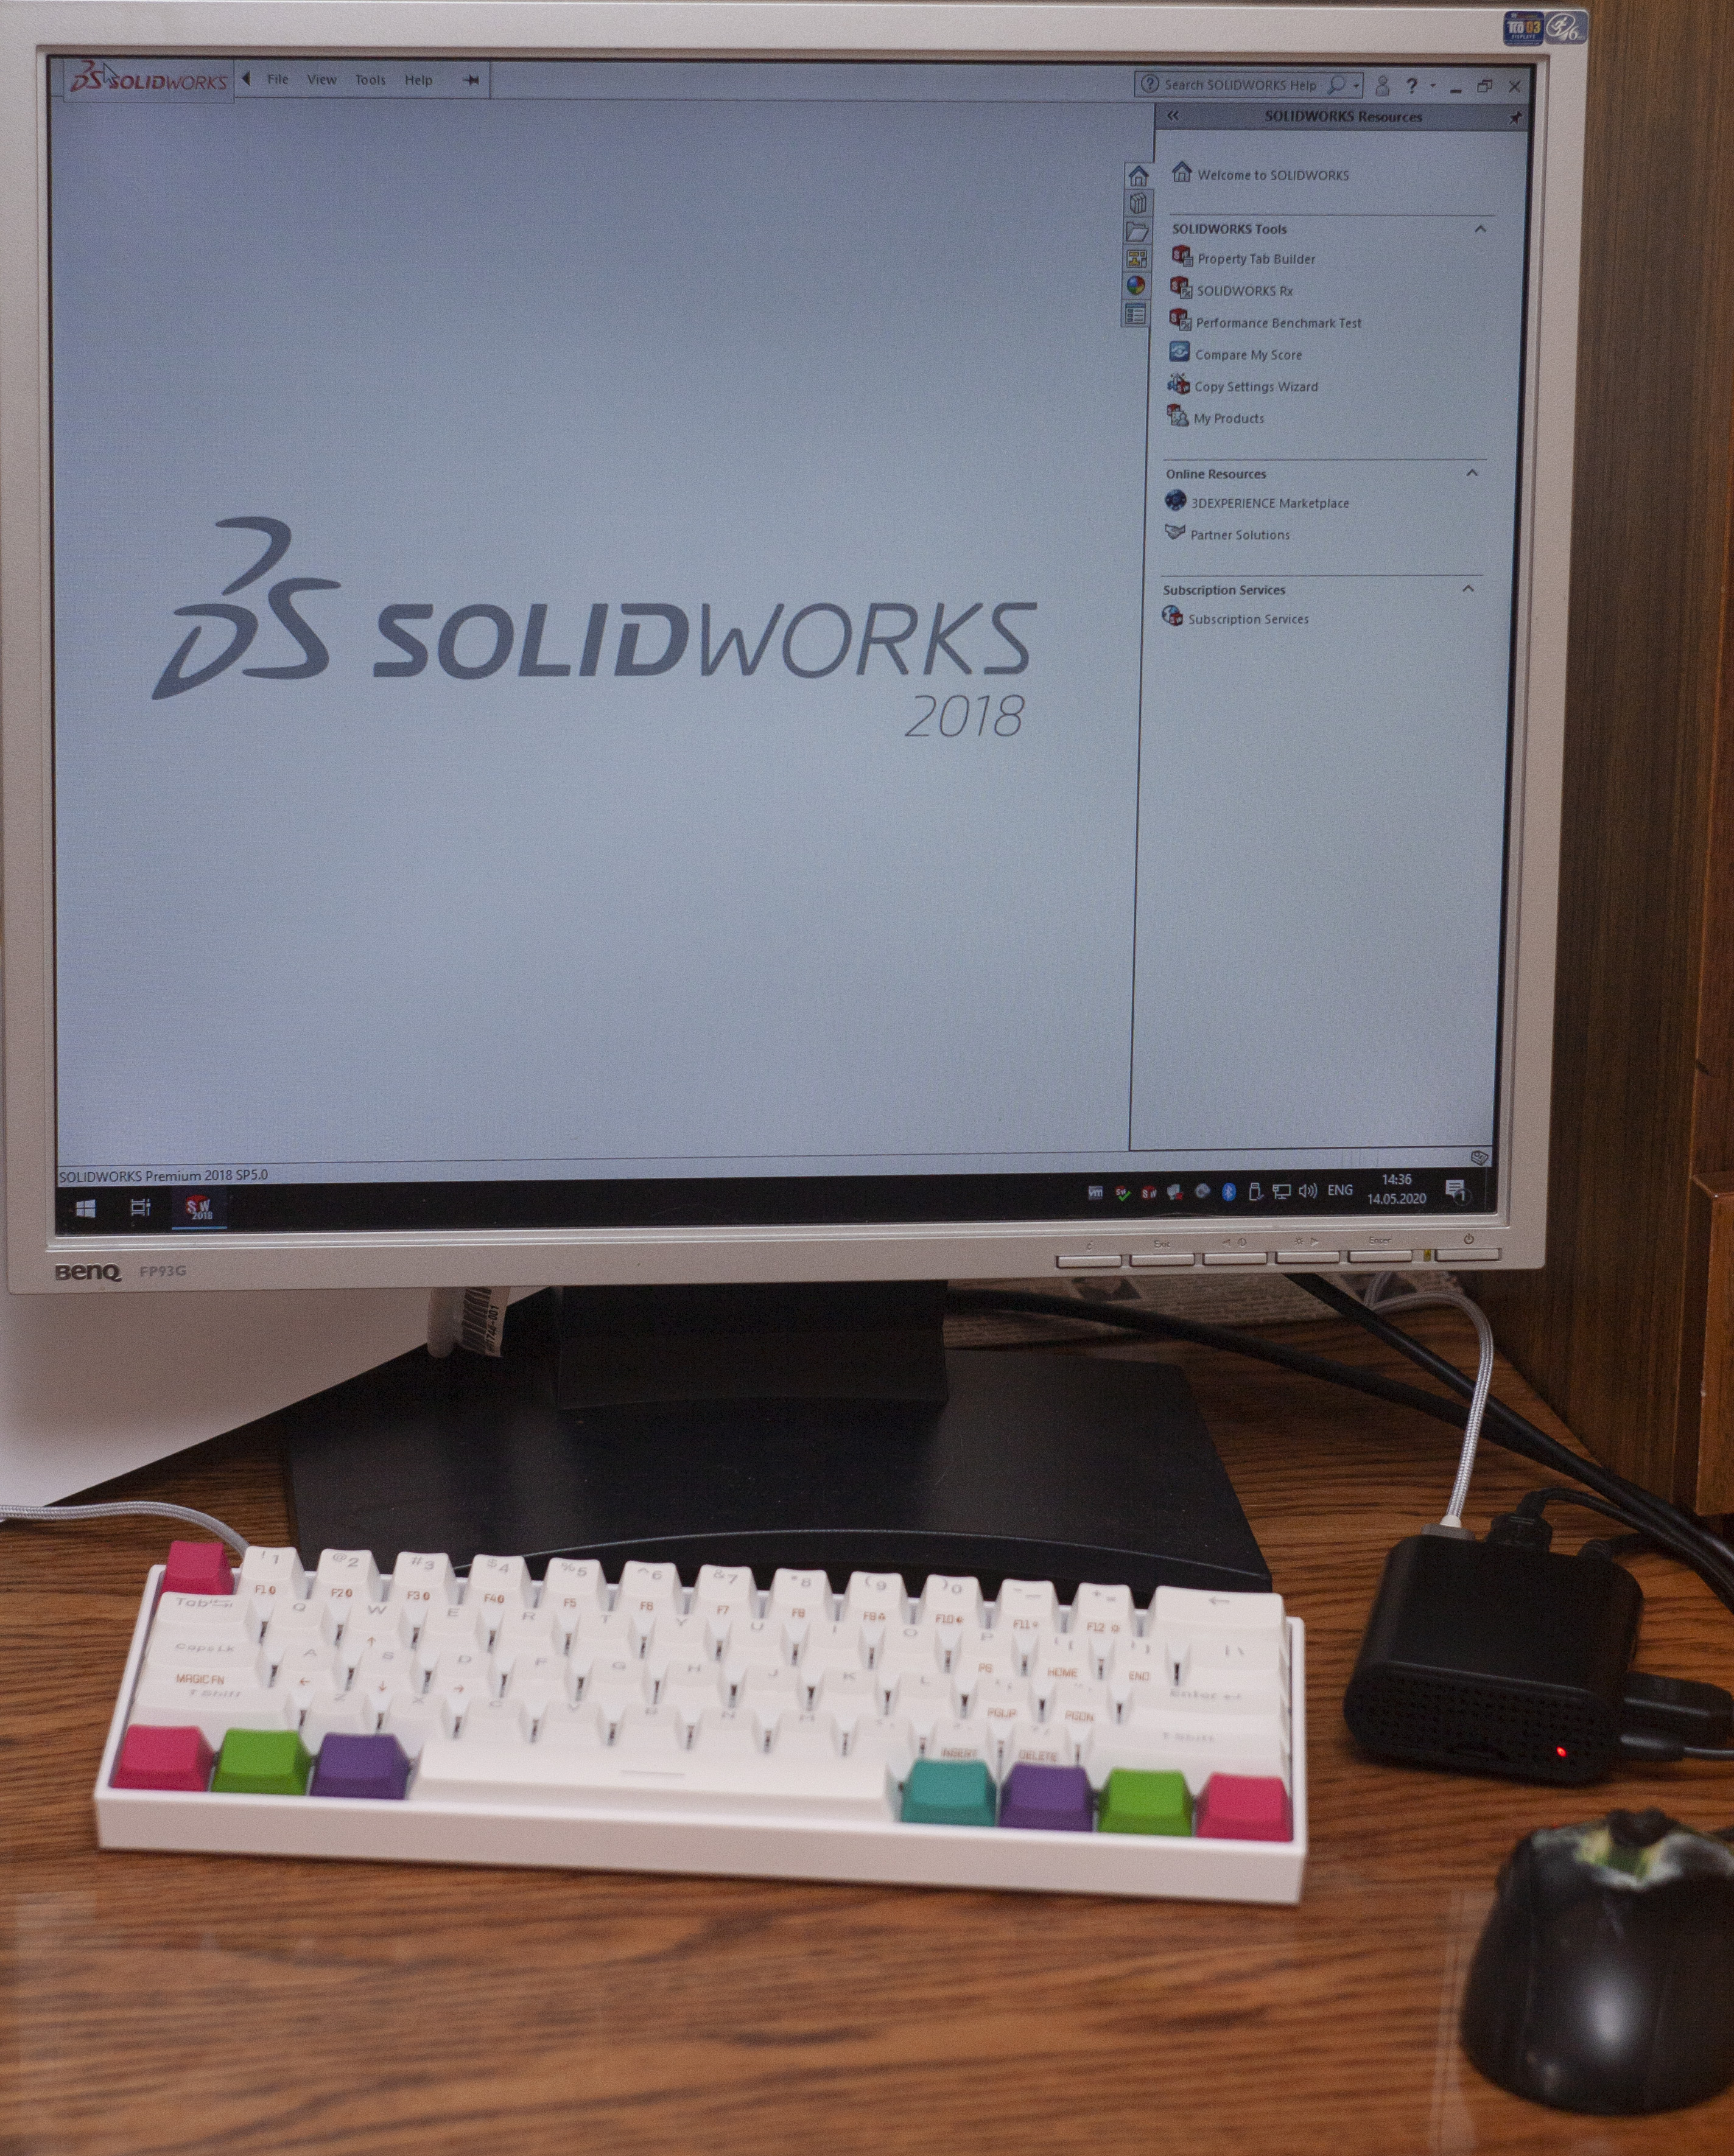
\includegraphics[width=\linewidth]{ph-solid}
    \caption{Готовый к работе тонкий клиент}
    \label{pic:ph-solid}
\end{figure}

Запускается RDP-клиент. Подключение к удаленному рабочему столу успешно (см.
рисунок~\ref{pic:ph-solid}). Завершается сеанс нажатием комбинации клавиш
Ctrl-Alt-Backspace. Осталось только прописать автоматическую загрузку сеанса. Для этого
в конец файла \texttt{~/.bash\_profile} нужно добавить следующую строку:
\begin{verbatim}
[[ -z $DISPLAY && $XDG_VTNR -eq 1 ]] && startx --
\end{verbatim}

После этого можно перезагрузить систему. После загрузки автоматически установится
RDP-соединение. Комбинация клавиш Ctrl-Alt-Backspace закрывает сеанс и возвращает в
консоль, это можно использовать при необходимости поменять конфигурацию. В графический
режим можно вернуться командой \texttt{startx --}, а комбинация клавиш Ctrl-D
перезапустит сеанс и так же загрузит графический режим.

\begin{figure}[h]
    \center
    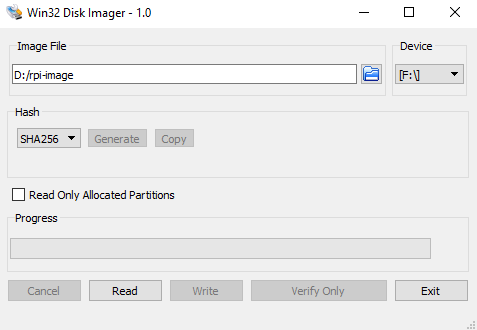
\includegraphics[width=\linewidth]{win32diskimager}
    \caption{Окно Win32 Disk Imager}
    \label{pic:win32di}
\end{figure}

Теперь с помощью программы Win32 Disk Imager \cite{ref:win32di} можно создать образ уже
настроенной системы, чтобы не настраивать каждый клиент отдельно. Далее можно будет на
карту памяти каждого клиента записать этот образ, после чего клиент будет готов к
работе. Останется только изменить логин и пароль пользователя в файле
\texttt{/etc/xdg/openbox/autostart}. Для создания такого образа нужно извечь карту
памяти из микрокомпьютера, вставить ее в ПК и открыть программу Win32 Disk Imager. В
окне нужно выбрать файл, в который будет записан образ системы, проверить соответствие
устройства и нажать кнопку Read (см. рисунок~\ref{pic:win32di}). Для уменьшения размера
образа можно воспользоваться опцией Read Only Allocated Partitions. Через некоторое
время образ будет считан. Теперь можно записывать его с помощью программ Etcher (так же,
как в начале установки) или Win32 Disk Imager (кнопка Write, затем Verify Only для
подтверждения корректности записи).

В дальнейшем при модернизации системы можно настроить TFTP-сервер, который позволит
загружать тонкие клиенты по сети, что позволит избавиться от неободимости в карте
памяти для каждого устройства и еще больше упростит конфигурацию новых клиентов. Однако
это увеличит время загрузки каждого клиента, т.к. придется скачивать весь образ по сети
при каждой загрузке.
